\documentclass[11pt]{article}

\usepackage[T1]{fontenc}
\usepackage{lmodern}
\usepackage[margin=1in]{geometry}
\usepackage{amsmath,amssymb}
\usepackage{booktabs}
\usepackage{graphicx}
\usepackage{xcolor}
\usepackage{listings}
\usepackage{url}
\usepackage[hidelinks]{hyperref}
\usepackage{microtype}
\usepackage{caption}
\usepackage[numbers,sort&compress]{natbib}

\lstset{
  basicstyle=\ttfamily\small,
  breaklines=true,
  columns=fullflexible,
  frame=single,
  framesep=4pt,
  xleftmargin=4pt,
  aboveskip=6pt,
  belowskip=6pt,
}

\setlength{\emergencystretch}{3em}
\newcommand{\pkg}[1]{\texttt{#1}}
\newcommand{\code}[1]{\texttt{#1}}

\title{How Much of Your Prompt Survives an Edit?\\
A Cross-Provider Measurement of Prompt-Cache Invalidation Granularity}

\author{Manas Vudugula\\
University of Florida\\
\texttt{manasvudugula@ufl.edu}}

\date{\today}

\begin{document}
\maketitle

\begin{abstract}
Prompt caching is now load-bearing for cost and latency in agentic LLM
applications, which routinely resend large, mostly-static tool and system
prefixes on every turn. Providers document \emph{that} caching exists, but
not precisely how invalidation is scoped: does a single edit anywhere in a
prefix wipe the whole cache, or does partial credit survive, and at what
granularity? We answer this directly, using each provider's own usage
telemetry (\code{cache\_read\_input\_tokens},
\code{prompt\_tokens\_details.\allowbreak cached\_tokens}, and DeepSeek's
\code{prompt\_cache\_hit\_tokens}) rather
than the timing side-channels used by prior work, and measure exactly how
many tokens of a shared prefix survive a single controlled perturbation,
across Anthropic, OpenAI, DeepSeek, and Gemini. We find four qualitatively
different regimes. Anthropic's granularity is entirely developer-controlled:
one \code{cache\_control} block is atomic (any edit is a full miss), while
splitting a static prefix from a variable tail gives perfect partial credit.
OpenAI and DeepSeek both cache in deterministic fixed-size chunks (1024 and
128 tokens respectively), confirmed by full positional sweeps and, on a
second, structurally different prefix, refined further: OpenAI's chunk
boundaries are content-anchored rather than fixed absolute-token addresses.
Gemini's realized cache credit is not a stable function of request content
at all: an isolated, byte-identical, repeated request returns different
credited-token counts across trials. Documented posture does not predict
measured reliability: DeepSeek's own documentation hedges caching as
``best-effort,'' while OpenAI's does not, yet DeepSeek is the most
deterministic provider we measure and Gemini, whose documentation carries no
comparable hedge, is the least. A length-changing-edit check (insertion
rather than substitution) finds no evidence of content-defined,
rolling-hash-style resync on any provider tested; every provider's behavior
is consistent with simple prefix/longest-common-prefix continuity, which
yields a concrete piece of practical guidance: append new content to the end
of a prefix rather than inserting it in the middle. ``Prompt caching'' is not
one mechanism; it is at least four different reliability contracts, and
cost or latency estimates that assume one provider's behavior generalizes to
another will be wrong.
\end{abstract}

\section{Introduction}

Agentic tool-calling systems resend the same large system prompt and tool
schema block on every turn of a conversation. Prompt caching, offered in some
form by every major LLM API provider, is the difference between re-billing
that entire block on every call and billing pennies for it after the first
turn. As agent frameworks grow more complex (more tools, longer system
prompts, deeper conversation histories), the fraction of a request that is
static, cacheable prefix keeps growing, and so does the cost consequence of
getting caching wrong.

What ``getting it wrong'' means in practice depends on a question providers'
documentation does not answer precisely: when a developer edits part of a
cached prefix (adds a tool, tweaks a system-prompt sentence, reorders a
parameter description), how much of the \emph{rest} of that prefix still
counts as cached? Is invalidation atomic (one edit anywhere kills the whole
cache), prefix-continuity-based (everything up to the edit survives,
everything after it does not), or something more forgiving, such as
content-defined chunking that can resync after the edited region? The answer
determines whether cache-aware prompt design is even possible for a given
provider, and if so, at what granularity a developer should think about it.

\paragraph{Prior art measures a shadow of this, not the thing itself.} The
closest existing work, \citet{prompt-cache-audit}, infers the presence of
prompt caching from response-latency side channels: cached requests return
faster, and a large enough sample of timing data reveals which providers
cache and roughly how. This is a real signal, but an indirect one. Timing is
noisy, requires statistical aggregation over many requests to separate
signal from network and inference-time variance, and, most importantly,
cannot directly report a \emph{magnitude}: it can suggest that some caching
happened, not read off exactly how many tokens of a specific edited prefix
were credited. We instead read the number directly, from the usage object
every provider already returns with every response.

\paragraph{Contributions.} This is a measurement paper, not a benchmark:
\begin{enumerate}
  \item The first direct-telemetry (not timing-inferred) cross-provider
  comparison of prompt-cache invalidation granularity, across Anthropic,
  OpenAI, DeepSeek, and Gemini (\S\ref{sec:results}).
  \item An empirical, corrected value for OpenAI's cache chunk size (1024
  tokens, not the commonly cited 128) from a systematic positional sweep, and
  a second provider, DeepSeek, whose chunk size does match the folklore
  128-token figure, showing the two numbers were never claims about the same
  system (\S\ref{sec:openai}, \S\ref{sec:deepseek}).
  \item A demonstration that Anthropic's granularity is a \emph{developer}
  choice, not a fixed provider constant: atomic with a single
  \code{cache\_control} block, perfect partial credit with the documented
  static/variable split (\S\ref{sec:anthropic}).
  \item Evidence that Gemini's automatic caching yields non-deterministic
  realized credit under an identical, isolated, repeated request, a
  reliability property distinct from granularity, contrasted directly with
  DeepSeek under the same isolation protocol, which returns bit-for-bit
  identical credit every time despite hedging more explicitly than any other
  provider's documentation (\S\ref{sec:gemini}).
  \item A methods note that Anthropic's OpenAI-compatibility shim silently
  drops all cache-accounting fields; only the native \code{/v1/messages} API
  exposes them, a trap for anyone benchmarking through the compatible
  surface (\S\ref{sec:method}).
  \item A methods note that DeepSeek's cache is disk-persisted and
  content-addressed globally, unlike Gemini's transient, replica-scoped
  cache, so the repeated-trial design that correctly surfaces Gemini's
  non-determinism silently self-contaminates on DeepSeek unless every
  repeated condition uses previously-unseen text (\S\ref{sec:method}).
  \item A generalization check on a second, structurally different prefix (a
  prose document, not a tool-schema list) that confirms three of the four
  provider characterizations unchanged and sharpens the fourth: OpenAI's
  chunk boundaries are content-anchored, not fixed absolute-token addresses
  (\S\ref{sec:generalization}).
  \item A cross-model-endpoint spot-check showing the same class of
  subtlety one layer down: DeepSeek's 128-token grain is a genuine platform
  constant shared between \code{deepseek-chat} and \code{deepseek-reasoner},
  but the two endpoints' chunk \emph{phase} differs, so a fixed nominal
  prefix position does not correspond to a fixed absolute token offset once
  model endpoint, not just prefix shape, varies (\S\ref{sec:bigmodel}).
  \item A length-changing-edit check (insertion, not substitution) that
  finds no evidence of content-defined, rolling-hash-style resync on any
  provider: credit is lost past an insertion point exactly as pure
  prefix-continuity caching predicts, direct evidence in favor of
  radix-tree-style KV-cache reuse over a content-defined-chunking
  alternative (\S\ref{sec:insertion}).
\end{enumerate}

\section{Background}
\label{sec:background}

Two caching designs are represented among the four providers we test.
Anthropic exposes explicit \code{cache\_control} breakpoints: a developer
marks specific content blocks as cacheable, and the provider caches
everything up to and including each marked block, giving the developer
direct control over granularity. OpenAI, DeepSeek, and Gemini instead cache
automatically: any sufficiently long request prefix is cached without any
special parameter, and the provider's own chunking logic determines what
counts as a reusable unit.

We use the following terms throughout. The \emph{prefix} is the shared,
mostly-static block of text sent as (part of) the system or leading user
content on every call. A \emph{perturbation} is a single controlled edit to
that prefix, at a known position, whose effect on caching we measure.
\emph{Credited tokens} are the token count a provider reports as served from
cache on a given call (\code{cache\_read\_input\_tokens},
\code{prompt\_tokens\_details.cached\_tokens}, or DeepSeek's
\code{prompt\_cache\_hit\_tokens}, depending on provider). The \emph{hit
fraction} is credited tokens divided by total prompt tokens. A \emph{chunk
boundary} is a position in the prefix past which an edit stops affecting
credited tokens for content before it, evidence of a discrete caching unit
rather than a single opaque block.

Two scope statements bound the study. First, we measure invalidation from
\emph{content edits}, not time-based cache expiration. Every provider we
test also imposes a time-to-live on cached content (Anthropic's default
five-minute ephemeral window is the most explicitly documented); TTL
behavior is a related but distinct question and is out of scope here.
Second, every measurement in this paper is of the author's own request
content, read via each provider's own accounting fields returned in response
to that same request. This is not a timing side-channel study, unlike
\citet{prompt-cache-audit}, and makes no attempt to infer or access any other
tenant's cached content.

\section{Method}
\label{sec:method}

\subsection{Test artifacts}
The primary test artifact is a synthetic tool-definition prefix: 45
templated tool schemas (a name, a description, and three parameters each),
totalling approximately 6,900--7,700 tokens depending on the provider's
tokenizer, chosen to be large enough to span
several cache chunks under every provider's minimum caching threshold
(OpenAI and Gemini require roughly 1024--2048 tokens; Anthropic, roughly
1024--2048 depending on model) and structurally representative of a real
agent's tool-calling system prompt. A second, structurally different
artifact, used for the generalization check in \S\ref{sec:generalization},
is a 45-section prose policy-handbook document of comparable total length
(approximately 5,600--7,700 tokens depending on model tokenizer) with no
tool schemas or parameter lists, so that any finding tied to the uniform
$\sim$155-token block structure of the tool-schema prefix can be
distinguished from a finding about the underlying caching mechanism itself.

\subsection{Perturbations}
Each perturbation is a single, deterministic edit at a controlled position,
so that the character offset of the first byte-level difference from the
unedited prefix is known exactly. The base perturbation set covers a
single-word edit in the header (position $\approx$0\%), a single-word edit
in the first block, a single-word edit at the midpoint block, a single-word
edit in the last block, a single trailing space appended after the full
prefix (position $\approx$100\%), and an adjacent-block swap at the midpoint
(a reorder rather than a substitution). Positional sweeps additionally place
a single-word substitution at every block index in turn (every tool, or
every section, from 1 to 45), which is how the chunk-boundary tables in
\S\ref{sec:openai}--\S\ref{sec:deepseek} were built. A separate
length-changing perturbation, an insertion of a new sentence rather than a
substitution, is described in \S\ref{sec:insertion}.

\subsection{Measurement protocol}
Every measurement follows the same three-call shape: a \emph{prime} call
sends the unedited prefix (populating the cache), a short gap elapses, and a
\emph{measurement} call sends a perturbed variant of the same prefix; the
credited-tokens field of the measurement call's response is read directly
from the provider's usage object. A byte-identical \emph{control} repeat
(no edit at all) is run alongside every perturbed condition to confirm the
cache is populated and behaving as expected before attributing a partial or
zero hit to the perturbation itself, rather than to a cold cache.

Per-provider protocol notes follow. \textbf{Anthropic} is queried via its
native \code{/v1/messages} endpoint rather than its OpenAI-compatible
\code{/v1/chat/completions} shim; the shim silently omits
\code{cache\_creation\_input\_tokens} and \code{cache\_read\_input\_tokens}
from its usage object even when the underlying \code{cache\_control}
directive is honored server-side, so anyone measuring Anthropic cache
behavior exclusively through the compatible surface would incorrectly
conclude the provider reports no cache statistics at all.
\textbf{OpenAI} results are collected primarily through OpenRouter, whose
\code{session\_id} parameter pins repeated calls to the same backend
instance; a direct-API cross-validation against \code{api.openai.com} is
reported in \S\ref{sec:crossvalidation}. \textbf{Gemini} required an
isolation protocol (\S\ref{sec:gemini}) once single-shot sweeps showed
variance under nominally identical conditions; the isolation control (one
fixed condition, repeated many times, with no other request touching the
API in between) rules out cross-condition test-harness leakage as an
alternative explanation. \textbf{DeepSeek}'s cache turned out to be
disk-persisted and content-addressed at the level of the whole API account,
not scoped to a session or a short TTL: any (position, exact-text) pair
sent even once becomes self-hittable indefinitely afterward. The
repeated-trial isolation design that correctly diagnosed Gemini's
non-determinism therefore silently self-contaminates on DeepSeek, since
every repeat after the first is a hit against the \emph{edited} variant's
own prior occurrence rather than an independent trial. Positional sweeps
against DeepSeek use single-shot, never-reused edit text at every position
for exactly this reason.

Inter-call gap timing (roughly 2.5--5 seconds, depending on the script) was
not held rigorously constant across every measurement script. We note this
rather than treat it as a confound: gap length is orthogonal to the
content-addressed and largely deterministic mechanisms measured here, and
every determinism/isolation check that specifically depends on timing
consistency (DeepSeek's isolation check, Gemini's isolation check) used one
fixed gap throughout its own run.

\section{Results}
\label{sec:results}

\subsection{Anthropic: developer-controlled granularity}
\label{sec:anthropic}
With the entire prefix in a single \code{cache\_control} block, any edit
anywhere, including a single trailing space appended after the full 6,900
tokens, produces a full cache miss: the block is atomic. Splitting the
prefix into a static, cache-marked block followed by an uncached variable
tail changes this completely. Table~\ref{tab:anthropic} shows the result on
both the tool-schema and prose-document prefixes: the static block is fully
credited regardless of what changes in the tail, giving perfect partial
credit by construction. Anthropic's granularity is therefore not a provider
constant to be measured at all; it is whatever granularity the developer
chooses to express via block boundaries.

\begin{table}[t]
\centering
\caption{Anthropic static-block-plus-tail structure. The static block is
fully credited (\code{cache\_read\_input\_tokens} equals the block's full
size) regardless of edits to the uncached tail, on both prefix shapes.}
\label{tab:anthropic}
\begin{tabular}{@{}lrrr@{}}
\toprule
Prefix shape & Static block size & Prime (cache write) & Repeat / edited tail (cache read) \\
\midrule
Tool-schema list & 7,590 tok & 7,590 & 7,590 \\
Prose document    & 5,672 tok & 5,672 & 5,672 \\
\bottomrule
\end{tabular}
\end{table}

\subsection{OpenAI: deterministic 1024-token chunks}
\label{sec:openai}
A full 45-position sweep on the tool-schema prefix (single-word
substitution at each tool index in turn, OpenAI's automatic caching, no
\code{cache\_control} equivalent needed) produced a clean, monotonic
staircase once four outlier readings were rechecked with fresh, isolated
calls (positions 1, 23, 36, and 45 initially returned values inconsistent
with their neighbors; a follow-up single-shot recheck at each resolved them
to the values shown in Table~\ref{tab:openai}, consistent with transient
session-routing noise on the initial sweep rather than a real effect).
The corrected result is six flat plateaus separated by five clean $+1024$
token steps, matching the prefix's total length of roughly 6,900 tokens
divided into six chunks of 1024 tokens each (the last, partial chunk credits
whatever remains); Figure~\ref{fig:openai-sweep} plots the same sweep as a
step function.

\begin{table}[t]
\centering
\caption{OpenAI chunk boundaries, tool-schema prefix, 45-position sweep
(corrected). Edit position is the index of the single tool block edited;
credited tokens is the corrected \code{cached\_tokens} reading for that
edit. Six flat plateaus, five clean $+1024$-token steps.}
\label{tab:openai}
\begin{tabular}{@{}lr@{}}
\toprule
Edit position (tool index) & Credited tokens \\
\midrule
1--12  & 0 \\
13--19 & 1{,}792 \\
20--25 & 2{,}816 \\
26--32 & 3{,}840 \\
33--39 & 4{,}864 \\
40--45 & 5{,}888 \\
\bottomrule
\end{tabular}
\end{table}

\begin{figure}[t]
\centering
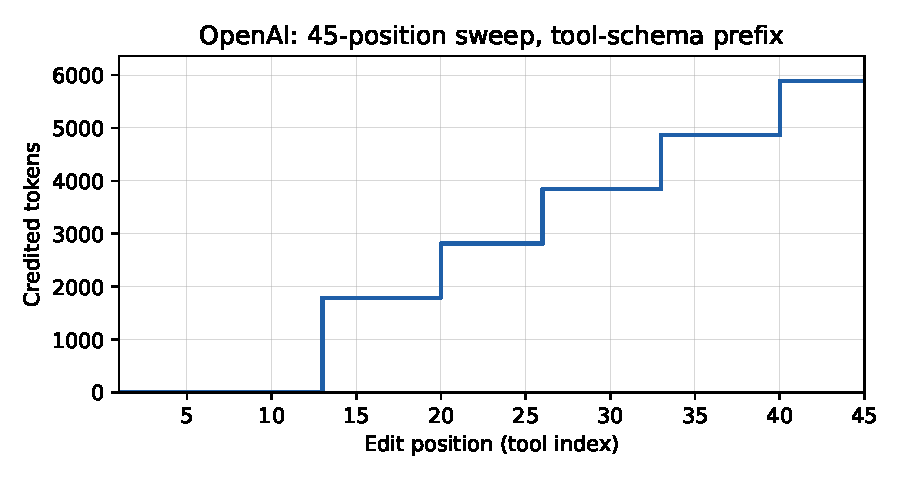
\includegraphics[width=0.72\linewidth]{figures/openai_sweep.pdf}
\caption{The same corrected 45-position sweep as Table~\ref{tab:openai},
plotted as a step function. Six flat plateaus, five clean $+1{,}024$-token
risers.}
\label{fig:openai-sweep}
\end{figure}

\subsection{DeepSeek: deterministic 128-token chunks despite a hedged spec}
\label{sec:deepseek}
DeepSeek's own documentation describes caching as best-effort and
explicitly does not guarantee a 100\% hit rate. Measured behavior is the
opposite of tentative. A 45-position single-shot sweep on the tool-schema
prefix (each position measured exactly once, for the self-contamination
reason described in \S\ref{sec:method}) produced a clean monotonic
staircase in which every single reading, without exception, is an exact
multiple of 128 tokens; Table~\ref{tab:deepseek} shows seven evenly-spaced
landmark positions from that sweep, independently rechecked with fresh,
single-shot calls, and Figure~\ref{fig:deepseek-sweep} plots the full
45-position staircase. Separately, an isolation check ran one fixed condition
eight times in a row: every one of the eight repeats returned exactly
7{,}040 of 7{,}055 credited tokens, zero variance. DeepSeek is, by this
measure, the most deterministic of the four providers tested, despite
carrying the most explicit hedge of any provider's documentation.

\begin{table}[t]
\centering
\caption{DeepSeek chunk boundaries, tool-schema prefix, seven landmark
positions from a 45-position single-shot sweep (independently rechecked).
Every value is an exact multiple of 128 tokens.}
\label{tab:deepseek}
\begin{tabular}{@{}lrr@{}}
\toprule
Edit position (tool index) & Credited tokens & Multiple of 128 \\
\midrule
1  & 0     & $0\times$ \\
8  & 1{,}152 & $9\times$ \\
16 & 2{,}304 & $18\times$ \\
24 & 3{,}584 & $28\times$ \\
32 & 4{,}864 & $38\times$ \\
40 & 6{,}016 & $47\times$ \\
45 & 6{,}784 & $53\times$ \\
\bottomrule
\end{tabular}
\end{table}

\begin{figure}[t]
\centering
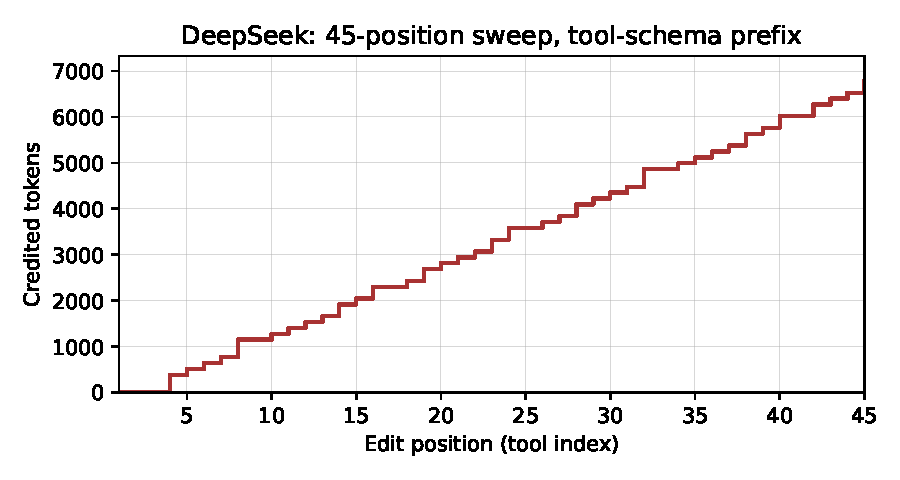
\includegraphics[width=0.72\linewidth]{figures/deepseek_sweep.pdf}
\caption{The full 45-position sweep underlying Table~\ref{tab:deepseek},
plotted as a step function. Every riser is an exact multiple of 128 tokens;
the seven landmark positions shown in the table sit on this same staircase.}
\label{fig:deepseek-sweep}
\end{figure}

\subsection{Gemini: unpredictable realized credit}
\label{sec:gemini}
Gemini's automatic caching is the outlier of the four providers on a
different axis entirely: not granularity, but reliability. A multi-position
sweep, repeated five times per position, shows per-position variance that
cannot be explained by the edit itself, since the edit is byte-identical
across repeats of the same condition (Table~\ref{tab:gemini}). To rule out
test-harness leakage (one condition's request somehow affecting another's
measured cache state) as an alternative explanation, an isolation control
ran a single fixed condition twelve times with no other request touching
the API in between. The variance persisted: the twelve repeats split across
three recurring values, 0, 3{,}061, and 7{,}143 credited tokens out of
7{,}694 total, in no discernible pattern.

\begin{table}[t]
\centering
\caption{Gemini cache-credit variance, tool-schema prefix, five repeats per
edit position (all positions share the same 7,694-token total). Distinct
values observed per position show that realized credit is not a stable
function of edit position, or of the request at all.}
\label{tab:gemini}
\begin{tabular}{@{}lll@{}}
\toprule
Edit position (tool index) & Distinct credited-token values observed (n=5) \\
\midrule
Control (no edit) & $\{0, 7{,}143\}$ \\
1  & $\{0, 7{,}143\}$ \\
8  & $\{0, 1{,}020, 7{,}143\}$ \\
16 & $\{2{,}041, 7{,}143\}$ \\
24 & $\{3{,}061, 7{,}143\}$ \\
32 & $\{0, 1{,}020, 5{,}102, 7{,}143\}$ \\
40 & $\{0, 6{,}123\}$ \\
45 & $\{6{,}123, 7{,}143\}$ \\
\bottomrule
\end{tabular}
\end{table}

This is the paper's clearest apples-to-apples determinism comparison:
the same isolation protocol, applied to Gemini and to DeepSeek
(\S\ref{sec:deepseek}), produces zero variance on one provider and
persistent variance on the other. The most parsimonious explanation is
unpinned load-balancing across backend replicas with independent cache
state and no client-facing session affinity, in contrast to, for example,
OpenRouter's explicit \code{session\_id} stickiness for OpenAI requests.

\section{Generalization Check: A Second Prefix Shape}
\label{sec:generalization}

Every result in \S\ref{sec:results} was measured on one prefix shape: a
list of uniform, near-identical $\sim$155-token tool schemas. A uniform
block prefix cannot distinguish fixed-address chunking (a chunk boundary
always falls at a specific token count from the start) from content-defined
chunking (a chunk boundary falls at a specific point determined by a
rolling hash of the content itself), because with uniformly-sized blocks
the two coincide. We reran the core measurements on the 45-section prose
document described in \S\ref{sec:method}, whose sections vary in length,
to break that degeneracy.

Three of the four provider characterizations reproduce unchanged.
Anthropic's static-block-plus-tail structure again gives perfect partial
credit (Table~\ref{tab:anthropic}, second row). DeepSeek's seven-position
sweep again produces a clean monotonic staircase in exact multiples of 128
tokens. Gemini's non-determinism not only reproduces but is starker: an
edit at section 1, immediately following the document header, still
returned 91\% cache credit (5{,}096 of 5{,}609 tokens) in two of three
repeats, underscoring that realized credit tracks something other than
edit position.

OpenAI's result reproduces at the magnitude level but reveals a sharper
mechanism. A seven-point sweep returned a reading of 1{,}792 credited
tokens at section 16, not a multiple of 1{,}024 as every prior OpenAI
reading had been. A full 45-position follow-up sweep (Table~\ref{tab:doc-openai})
resolved the anomaly: inter-boundary spacing is still exactly $+1{,}024$
tokens across three consecutive confirmed steps, but the \emph{first}
boundary is not aligned to a multiple of 1{,}024 tokens from the start of
the prefix, something never observed on the uniform tool-schema prefix. The
most parsimonious interpretation is that OpenAI's chunk boundaries are
content-anchored (consistent with rolling-hash, content-defined chunking
targeting roughly 1{,}024 tokens per chunk) rather than fixed absolute-token
addresses. The tool-schema prefix's uniform block size made this
indistinguishable from fixed-address chunking; the document's non-uniform
section lengths exposed it. This refines, rather than contradicts, the
finding in \S\ref{sec:openai}.

\begin{table}[t]
\centering
\caption{OpenAI chunk boundaries, prose-document prefix, 45-position sweep.
Inter-boundary spacing is a clean $+1{,}024$ tokens, but the first boundary
(position 16, 1{,}792 credited tokens) is not itself a multiple of 1{,}024
from the prefix start, unlike every boundary observed on the uniform
tool-schema prefix (Table~\ref{tab:openai}).}
\label{tab:doc-openai}
\begin{tabular}{@{}lr@{}}
\toprule
Edit position (section index) & Credited tokens \\
\midrule
1--15  & 0 \\
16--23 & 1{,}792 \\
24--32 & 2{,}816 \\
33--40 & 3{,}840 \\
41--45 & 4{,}864 \\
\bottomrule
\end{tabular}
\end{table}

Headline: three of four provider characterizations generalize unchanged
across prefix shape; OpenAI's generalizes at the magnitude level but
reveals a more precise mechanism, content-anchored rather than
fixed-address chunking, only visible on a non-uniform prefix. This is
itself a methodological point: a synthetic prefix built from uniform blocks
can hide the true chunking mechanism behind an aliasing artifact, so
measurement papers using synthetic prefixes should vary block-size
uniformity, not just block count or position.

\section{OpenAI Cross-Validation: OpenRouter versus Direct API}
\label{sec:crossvalidation}

Every OpenAI result reported above was measured through OpenRouter's
OpenAI-compatible proxy rather than \code{api.openai.com} directly, an
unresolved confound: OpenRouter could in principle add its own routing or
session logic that alters the numbers it passes through. We obtained a
direct OpenAI API key and reran the same seven landmark positions from the
prose-document sweep directly against \code{api.openai.com}, comparing
against the existing OpenRouter measurements as ground truth
(Table~\ref{tab:crossval}). All seven positions matched exactly, including
the total prompt token count (5{,}587 in both), indicating that OpenRouter
passes OpenAI's cache telemetry through unmodified for this model and
prefix.

\begin{table}[t]
\centering
\caption{OpenAI direct-API cross-validation against OpenRouter, seven
landmark positions, prose-document prefix. Exact match on all seven,
including total prompt tokens (5,587 both routes).}
\label{tab:crossval}
\begin{tabular}{@{}lrr@{}}
\toprule
Edit position (section index) & OpenRouter (reference) & Direct API \\
\midrule
1  & 0     & 0 \\
8  & 0     & 0 \\
16 & 1{,}792 & 1{,}792 \\
24 & 2{,}816 & 2{,}816 \\
32 & 2{,}816 & 2{,}816 \\
40 & 3{,}840 & 3{,}840 \\
45 & 4{,}864 & 4{,}864 \\
\bottomrule
\end{tabular}
\end{table}

Reaching the direct API required two request-shape changes that
OpenRouter's compatibility layer silently absorbs: the tested model
(\code{gpt-5-mini}) rejects the \code{max\_tokens} parameter directly
(only \code{max\_completion\_tokens} is accepted), and rejects any explicit
\code{temperature} value other than the model's default. Both are minor
in isolation, but worth recording, since either would produce a confusing
hard failure for anyone porting a measurement harness from OpenRouter to
the direct API without first checking provider-specific parameter support.

\section{Larger-Model Spot-Checks}
\label{sec:bigmodel}

Every result above uses one model per provider family
(\code{claude-haiku-4-5}, \code{gpt-5-mini}, \code{deepseek-chat},
\code{gemini-2.5-flash}). To address, cheaply rather than by leaving purely
as an admitted gap, whether these findings hold at a larger or
differently-architected model within the same provider, we ran targeted
(not systematically swept) spot-checks on a bigger model per provider,
using the prose-document prefix (Table~\ref{tab:bigmodel}).

\begin{table}[t]
\centering
\caption{Larger-model spot-checks against the small-tier reference, prose-document
prefix. Anthropic and OpenAI reproduce exactly. DeepSeek's chunk size holds
but its boundary phase shifts. Gemini's pro-tier result is reported as
inconclusive, not as evidence of determinism (see text).}
\label{tab:bigmodel}
\small
\begin{tabular}{@{}llrr@{}}
\toprule
Provider & Larger model & Result & Small-tier reference \\
\midrule
Anthropic & \code{claude-opus-4-8}    & 8{,}374 / 8{,}374 (full credit) & 8{,}374 / 8{,}374 (full credit) \\
OpenAI    & \code{gpt-5} (full)       & 2{,}816 (section 24)           & 2{,}816 (section 24) \\
DeepSeek  & \code{deepseek-reasoner}  & 2{,}816 (section 24)           & 1{,}792 (section 24) \\
Gemini    & \code{gemini-3.1-pro-preview} & 0/0/0 (3 reps, section 24) & 0/0/2{,}038 (3 reps, section 24) \\
\bottomrule
\end{tabular}
\end{table}

Anthropic and OpenAI reproduce their small-tier behavior exactly: the
larger Anthropic model still gives full partial credit on the static
block, and the larger OpenAI model lands on precisely the same chunk
boundary as \code{gpt-5-mini} at the same edit position. DeepSeek does not
reproduce exactly, but not randomly either: at all four positions tested
(8, 16, 24, and 40), \code{deepseek-reasoner} credits systematically more
than \code{deepseek-chat} at the same nominal position, yet every single
reading on both models, without exception, remains an exact multiple of
128 tokens (Table~\ref{tab:deepseek-multipos}). The most likely
explanation is that the 128-token grain is a genuine platform constant
shared across DeepSeek's model endpoints, but the chunk \emph{phase}, where
the first boundary falls, differs between \code{deepseek-chat} and
\code{deepseek-reasoner}, plausibly because the reasoner endpoint prepends
a different amount of hidden scaffolding to the prompt, shifting where a
given nominal prefix position lands in the model's actual token stream.
This parallels the content-anchored-boundary finding in
\S\ref{sec:generalization}: a uniform position index is not equivalent to
an absolute token offset once model endpoint, not just prefix shape,
varies.

\begin{table}[t]
\centering
\caption{DeepSeek cross-endpoint spot-check, four positions, prose-document
prefix. \code{deepseek-reasoner} credits systematically more than
\code{deepseek-chat} at the same nominal position, but both remain exact
multiples of 128 tokens throughout.}
\label{tab:deepseek-multipos}
\begin{tabular}{@{}lrrr@{}}
\toprule
Edit position (section index) & \code{deepseek-chat} & \code{deepseek-reasoner} & Delta \\
\midrule
8  & 0     & 896   & $+896$ \\
16 & 896   & 1{,}792 & $+896$ \\
24 & 1{,}792 & 2{,}816 & $+1{,}024$ \\
40 & 3{,}840 & 4{,}864 & $+1{,}024$ \\
\bottomrule
\end{tabular}
\end{table}

Gemini's pro-tier check returned zero variance across three repeats at
section 24 (0/0/0), contrasting with flash's variance at the same position
in the doc-shape sweep (0/0/2{,}038 across three repeats). We report this
cautiously and do not read it as evidence that the pro tier is more
deterministic: three repeats is a much smaller sample than the twelve-rep
isolation check that established flash's non-determinism in
\S\ref{sec:gemini}, so an absence of variance in three trials is
consistent with either a genuinely more stable pro-tier backend or simply
not having sampled enough to see the same variance flash shows. We flag
this as an open question rather than a claim.

Reaching the larger tiers surfaced two further direct-API parameter
quirks: \code{claude-opus-4-8} rejects the \code{temperature} parameter
outright (``deprecated for this model,'' a different rejection reason than
\code{gpt-5}'s in \S\ref{sec:crossvalidation}), and both
\code{gemini-2.5-pro} and \code{gemini-3-pro-preview} were already
deprecated and unavailable to new API keys by the time of testing, despite
being listed by the provider's own models endpoint; \code{gemini-3.1-pro-preview}
was used instead.

\section{Length-Changing Edits: Insertion, Not Just Substitution}
\label{sec:insertion}

Every perturbation up to this point has been a same-length word
substitution. Real prompt edits (adding a new tool, extending a parameter
description) are often insertions that shift the absolute token offset of
everything downstream of the edit, untested until this point, and the
natural next question raised by the content-anchored-boundary
(\S\ref{sec:generalization}) and endpoint-phase-shift (\S\ref{sec:bigmodel})
findings: does a length-changing edit let downstream content
\emph{resync} with the cache once the edited region has passed, evidence of
true content-defined, rolling-hash-style chunking, or is credit lost
entirely past the insertion point, consistent with pure prefix or
longest-common-prefix continuity caching, as used by radix-tree-style
KV-cache reuse systems?

We inserted one new sentence at the end of section 16 of the prose-document
prefix (appending to the section's existing text rather than replacing any
of it) and compared the resulting credited-token count against a same-position
substitution reference.

\paragraph{A methods note on choosing the right reference.} The naive
choice of reference, a substitution at the \emph{start} of section 16, is
not an apples-to-apples comparison, because the insertion appends new text
after the section's complete original content, so its actual
byte-level divergence point from the unedited prefix falls later than a
substitution in that section's first sentence would. This was caught during
analysis: an initial DeepSeek reading of 1{,}792 credited tokens for the
insertion looked, against the naive start-of-section reference of 896,
like evidence of resync (credit \emph{above} the reference). A corrected
reference, a substitution in section 16's \emph{last} sentence, matching
the insertion's true divergence point, gave 1{,}920, and 1{,}792 sits below
that corrected reference; the apparent resync evidence evaporated once the
comparison was fixed. We report this as a methods-section finding in its
own right: comparing edit conditions on cache credit requires matching the
actual byte-divergence offset, not just the nominal section or block
index, or a valid-looking effect can appear from a mismatched baseline
alone.

\begin{table}[t]
\centering
\caption{Insertion versus corrected (end-of-section) substitution
reference, section 16, prose-document prefix. Both providers land at or
below their reference, with no evidence of downstream resync.}
\label{tab:insertion}
\begin{tabular}{@{}lrr@{}}
\toprule
Provider & Insertion (credited tokens) & End-of-section substitution reference \\
\midrule
OpenAI (direct API) & 1{,}792 & 1{,}792 \\
DeepSeek             & 1{,}792 & 1{,}920 \\
\bottomrule
\end{tabular}
\end{table}

With the corrected reference in place (Table~\ref{tab:insertion}), neither
provider shows resync evidence. OpenAI's insertion result exactly matches
both the start- and end-of-section substitution references, because
sections 16 through 23 form a single flat plateau on OpenAI's coarser,
content-anchored chunk grain (\S\ref{sec:generalization},
\S\ref{sec:crossvalidation}): any edit within that span, insertion or
substitution, produces the same reading regardless of exactly where within
the span it falls. DeepSeek's insertion result sits slightly \emph{below}
the corrected reference, exactly as pure prefix-continuity caching
predicts: the extra tokens introduced by the insertion shift everything
after it just far enough to fall short of the next 128-token chunk
boundary that the same-length substitution reached.

Gemini's three insertion repeats returned $\{0, 5{,}096, 5{,}096\}$; 5{,}096
is the same near-full-credit value that recurs across multiple unrelated
conditions throughout this study's Gemini data (the control condition,
section-1 edits, section-45 edits in \S\ref{sec:generalization}),
reinforcing rather than adding to the existing non-determinism finding:
Gemini's realized credit does not track the edit's content, position, or
length, only which backend replica happened to answer. Anthropic was not
retested here, since its \code{cache\_control} mechanism is fully
developer-explicit at block granularity and cannot be affected by an
edit's length; it is already fully characterized in \S\ref{sec:anthropic}
and \S\ref{sec:generalization}.

\paragraph{Headline.} No evidence of content-defined, rolling-hash-style
resync on any provider tested. Length-changing edits behave exactly as
pure prefix-continuity caching predicts, consistent with, though not
direct proof of, radix-tree-style KV-cache reuse as the underlying
mechanism on OpenAI and DeepSeek. The practical implication carried into
\S\ref{sec:discussion} is concrete: appending new content to the very end
of a prefix is strictly safer than inserting it mid-prefix, which costs at
least as much cache credit as an equivalent substitution and never
recovers any of it downstream, on every provider tested.

\section{Discussion}
\label{sec:discussion}

\paragraph{Cache-aware prefix design is provider-specific.} For agent
framework authors, cache-aware prefix design is possible and fully
effective on Anthropic, since the developer controls the granularity
directly; free but coarse on OpenAI and DeepSeek, where aligning edits to
the roughly 1{,}024- or 128-token chunk boundary matters if cost is a
concern; and not reliable on Gemini regardless of how the prefix is
structured. Cost-estimation tooling that assumes a fixed hit rate per
provider will be systematically wrong specifically for Gemini, not merely
imprecise.

\paragraph{Documented posture does not predict measured behavior.} The
provider whose documentation carries the strongest hedge, DeepSeek's
explicit ``best-effort, does not guarantee 100\% hit rate,'' is the most
deterministic provider we measure. The provider with no comparable hedge,
Gemini, is the least reliable. A developer choosing a caching strategy
based on provider documentation alone, rather than direct measurement,
would draw the opposite conclusion from the truth for at least these two
providers.

\paragraph{The compatibility-shim telemetry gap is a trap.} Anyone
building cross-provider cache observability on top of an
OpenAI-compatible surface, a natural choice given how many providers
expose one, will silently lose Anthropic's cache statistics specifically,
since they are omitted from the compatible endpoint's usage object even
though the underlying caching itself is working correctly.

\paragraph{Experimental design does not transfer across providers
untouched.} The repeated-trial protocol that correctly diagnosed Gemini's
non-determinism produces a false-positive determinism reading on DeepSeek
if applied without first understanding that DeepSeek's cache is
persistent and content-keyed rather than session-scoped. Measurement
methodology itself needs to be adapted per provider, not assumed portable.

\paragraph{A uniform-block prefix can hide mechanism.} OpenAI's 1{,}024-token
finding held at the magnitude level on a non-uniform prefix
(\S\ref{sec:generalization}), but the boundary alignment shifted, revealing
content-anchored rather than fixed-address chunking that the uniform
tool-schema prefix could not have exposed. Future measurement work using
synthetic prefixes should vary block-size uniformity deliberately, not
just block count or edit position, to avoid mistaking a chunking artifact
of the test prefix for the provider's true mechanism.

\paragraph{Append, don't insert.} A specific, actionable recommendation
falls out of \S\ref{sec:insertion}: adding new content at the very end of
a prefix costs nothing beyond the new content itself, while inserting it
mid-prefix, for example adding a new tool in the middle of an existing
tool list, costs at least as much cache credit as editing that same spot,
and never recovers any of it downstream, however far past the insertion
point the following content is identical to what was cached before, on
every provider tested. Agent frameworks that expect to add tools or
context over a session's lifetime should append rather than insert
whenever the two are otherwise equivalent.

\section{Threats to Validity and Limitations}
\label{sec:limitations}

We are deliberate about the scope of the empirical claims.

\textbf{(1) Two synthetic prefix shapes, both surrogates.} We test a
tool-schema list and a prose document, chosen to be structurally different
enough to expose a mechanism the first shape alone could not
(\S\ref{sec:generalization}). Both remain synthetic surrogates for real
agent system prompts and may not generalize to other structures found in
production systems, such as few-shot examples or retrieved-chunk RAG
contexts with heterogeneous source formatting.

\textbf{(2) One model per provider family, spot-checked against a larger
model.} Primary results use one small/fast model per provider
(\code{claude-haiku-4-5}, \code{gpt-5-mini}, \code{deepseek-chat},
\code{gemini-2.5-flash}). \S\ref{sec:bigmodel} spot-checks, rather than
systematically sweeps, a larger or differently-architected model per
provider: Anthropic and OpenAI reproduced identically; DeepSeek's chunk
size held but its boundary phase shifted between endpoints; Gemini's
pro-tier determinism remains genuinely untested at the sample size that
would be needed to draw a conclusion, only three repeats were run, against
twelve for the isolation check that established flash's non-determinism.

\textbf{(3) Point-in-time characterization.} Gemini's non-determinism and
DeepSeek's determinism are characterized as of the testing period
(July 2026); provider-side infrastructure changes could alter, improve, or
degrade either at any time without notice, since none of this behavior is
part of any provider's documented contract.

\textbf{(4) Self-reported telemetry.} We have no access to provider-internal
ground truth. Every credited-token figure in this paper is trusted as
accurate but is still self-reported by the provider being measured; a
provider that misreported its own cache statistics (for reasons unrelated
to the caching behavior itself) would not be detectable by this method.

\textbf{(5) OpenAI measured primarily through a proxy.} The bulk of OpenAI
results in \S\ref{sec:openai} and \S\ref{sec:generalization} were
collected through OpenRouter rather than directly against
\code{api.openai.com}. \S\ref{sec:crossvalidation} cross-validates seven
landmark positions directly and finds an exact match, which we take as
reasonably strong evidence against a routing-introduced confound for this
model and prefix, but the cross-validation itself covers only seven of the
45 swept positions, not the full sweep.

\section{Conclusion}

Prompt caching is not one mechanism. Across four major providers we
measure four different reliability contracts: fully developer-controlled
on Anthropic, deterministic but coarse-grained and content-anchored on
OpenAI, deterministic and fine-grained on DeepSeek despite the most
cautious documentation of the four, and simply unreliable on Gemini
regardless of prefix structure. These were measured directly, from each
provider's own usage telemetry, rather than inferred from response
timing, and the resulting numbers (chunk sizes, hit-fraction variance, and
the behavior of length-changing edits) are precise enough to inform
concrete prefix-design decisions, most directly the recommendation to
append rather than insert. Cost and latency estimates for agentic LLM
systems that assume one provider's caching behavior generalizes to
another will be wrong, and the size of that error is largest for anyone
building on Gemini while assuming Anthropic- or DeepSeek-like reliability.

% -----------------------------------------------------------------------------
\begin{thebibliography}{9}

\bibitem[Gu et al.(2025)]{prompt-cache-audit}
Chenchen Gu, Xiang Lisa Li, Rohith Kuditipudi, Percy Liang, and Tatsunori
Hashimoto. Auditing Prompt Caching in Language Model APIs. \emph{ICML},
2025. arXiv:2502.07776.

\end{thebibliography}

\appendix
\section{Reproducibility}
All measurement scripts are pure-standard-library Python (\pkg{urllib} for
HTTP, no third-party dependencies beyond an \code{.env} loader), organized
as one script per provider/check, each writing its raw results to an
adjacent JSON file. Representative entry points:
\begin{lstlisting}
# Anthropic static-block-plus-tail structure (tool-schema and doc-shape prefixes)
python test_anthropic_multiblock.py
python doc_multiblock_anthropic.py

# OpenAI / DeepSeek 45-position chunk-boundary sweeps
python sweep_chunk_boundary.py          # OpenAI, tool-schema prefix
python deepseek_full_sweep.py           # DeepSeek, tool-schema prefix
python doc_full_sweep_openai.py         # OpenAI, prose-document prefix

# Gemini / DeepSeek isolation (determinism) checks
python gemini_isolation_check.py
python deepseek_isolation_check.py

# OpenAI direct-API cross-validation, larger-model spot-checks,
# and the insertion/length-changing-edit check
python openai_direct_validation.py
python bigmodel_anthropic.py bigmodel_openai.py bigmodel_deepseek.py bigmodel_gemini.py
python openai_insertion_check.py deepseek_insertion_check.py gemini_insertion_check.py
\end{lstlisting}
Each script's corresponding \code{*\_results.json} file, referenced by name
throughout \S\ref{sec:results}--\S\ref{sec:insertion}, contains the raw
provider usage object for every call made, sufficient to recompute every
table and figure in this paper without rerunning any API calls.
\code{make\_figures.py} regenerates Figures~\ref{fig:openai-sweep} and
\ref{fig:deepseek-sweep} directly from \code{chunk\_sweep\_results.json},
\code{recheck\_sweep\_outliers.json}, \code{deepseek\_full\_sweep\_}
\code{results.json}, and \code{deepseek\_recheck\_outliers.json}.

\end{document}
